\documentclass[12pt,onecolumn,a4paper]{article}
\usepackage{epsfig,graphicx,amsthm,amsmath}
\usepackage{color,xcolor}
\usepackage{pgfplots}
\pgfplotsset{compat=newest}
\usepackage{tikz}
\usepackage{caption}
\usepackage{subcaption}
\usepackage{xepersian}
\settextfont{XB Zar}
\setlatintextfont{Times New Roman}

\newtheorem{theorem}{قضیه}[section]
\newtheorem{corollary}{نتیجه‌}[theorem]

\pgfplotstableread[col sep = comma]{gibbs.csv}\gibbs
\pgfplotstableread{
-1 0
-1 -1
0 -1
0 1
1 1
1 0
}\gibbsref

\begin{document}
\title{توجیه وجود مثال‌های خصمانه \\ و انتقال‌پذیری آن‌ها} 
\author{رامین براتی}
\date{\today}
\maketitle

\begin{abstract}
چکیده
\end{abstract}

\section{مقدمه} 
مقدمه.

\section{کارهای مرتبط}
تاکنون، برای وجود مثال‌های خصمانه سه دلیل ارائه شده است. اولین دیدگاه توسط سجدی و همکاران
(مقاله)
مطرح شد. این دیدگاه، که با نام دیدگاه پاکت‌های نادر شناخته می‌شود، به شرح زیر است. در این دیدگاه، دلیل وجودی مثال‌های خصمانه وجود پاکت‌هایی در فضای ورودی شبکه هستند که احتمال مشاهده‌ی آنها بسیار کم است و شبکه در آن نواحی خروجی مناسبی نمی‌دهد. در این دیدگاه رابطه‌ی مثال‌های خصمانه با فضای ورودی شبکه را مشابه رابطه‌ی میان اعداد گویا و اعداد حقیقی می‌دانند. به این معنی که، احتمال گویا بودن یک نمونه‌ی تصادفی از یک بازه از اعداد حقیقی صفر است، با این وجود در همسایگی هر عدد حقیقی عددی گویا یافت می‌شود. با این حال،
همان گونه که در
(مقاله)
نیز به آن اشاره شده است، دلیل محکمی برای نشان دادن چنین رفتاری توسط شبکه ارائه نشده است و صرفا به مرتبط کردن آن به بسیار غیرخطی بودن نمایش یادگیری شده توسط شبکه اکتفا شده است. این دیدگاه چگونگی انتقال این مثال‌ها به شبکه‌های دیگر را نیز مشخص نمی‌کند.

دیدگاه دوم توسط گودفلو و همکاران
(مقاله)
مطرح شده است. این دیدگاه، که با نام دیدگاه خطی بودن شناخته می‌شود، هم اکنون مقبول‌ترین دیدگاهی است که در این زمینه ارائه شده است. طبق این دیدگاه، پدیده‌ی مثال‌های خصمانه در طبقه‌بندهای خطی در ابعاد بالا ظهور می‌کند و دلیل مشاهده‌ی این پدیده در شبکه‌های عصبی نیز مرتبط با علاقه‌ی ما در استفاده از الگوهای خطی در مدلسازی و آموزش این شبکه‌ها می‌باشد. گودفلو و همکاران با استفاده از این دیدگاه حمله‌ی
\lr{FGSM}
را طراحی کردند که از این خطی بودن شبکه‌های عصبی برای تولید مثال‌های خصمانه استفاده می‌کند. طبق این دیدگاه، دلیل انتقال مثال‌های خصمانه به دیگر شبکه‌ها را همگرایی این مدل‌ها به طبقه‌بند خطی بهینه می‌داند. دیدگاه خطی بودن دو پیش بینی مستقیم دارد، اول این که تمامی طبقه‌بندهای خطی از پدیده‌ی مثال‌های خصمانه رنج می‌برند و دوم این که اثر خطی بودن با افزایش ابعاد مسئله تشدید می‌شود. با این وجود، در
(مقاله)
هر دوی این پیش بینی‌ها زیر سوال می‌روند. ابتدا مسئله‌ای  مصنوع را در نظر می‌گیرند که برای آن طبقه‌بند خطیی وجود دارد که از مثال‌های خصمانه آزاد است و در ادامه نشان می‌دهند که در یک مسئله‌ی واقعی نیز با افزایش ابعاد قدرت مثال‌های خصمانه تشدید نمی‌شود.

دیدگاه سوم توسط تانای و همکاران
(مقاله)
 و با نام دیدگاه کجی مرز ارائه شده است. این دیدگاه برای طبقه‌بندهای خطی پیشنهاد شده و ظهور آن در شبکه‌های عصبی را منتج از شکلی غیرخطی از این پدیده می‌دانند. یک مسئله‌ی طبقه‌بندی دو کلاسی را در نظر بگیرید که برای آن یک طبقه‌بند خطی را آموزش داده‌ایم. این طبقه‌بند خطی یک مرز تصمیم
 $c$
 برای جدا کردن دو کلاس می‌یابد. حال طبقه‌بند بهینه‌ای را برای همان مسئله در نظر بگیرید که توسط مرکزهای دو کلاس تعریف شده باشد. این طبقه‌بند نیز یک مرز تصمیم
 $c^*$
 برای جدا کردن دو کلاس تعریف می‌کند. طبق دیدگاه کجی مرز در صورتی که مرز
 $c$
 با
 $c^*$
 زاویه داشته باشد، برای طبقه‌بند مثال‌های خصمانه وجود خواهد داشت. تانای و همکاران در ادامه نشان می‌دهند که می‌توان زاویه‌ی بین دو مرز را با منظم کردن\LTRfootnote{regularize}
طبقه‌بند کاهش داد. در پایان، تانای و همکاران با توجه به نوع و شکل اختلالات خصمانه‌ای که در شبکه‌های عصبی مشاهده می‌کنند، دلیل وجود مثال‌های خصمانه برای این شبکه‌ها را منظم نبودن این شبکه اعلام می‌کنند. با این که تانای و همکاران دلایل خوبی در تایید دیدگاه کجی مرز ارائه می‌دهند، چگونگی تعمیم آن به شبکه‌های عصبی و دیگر مدل‌های غیرخطی را مشخص نمی‌کنند. همچنین، در این دیدگاه دلیلی برای انتقال‌پذیری مثال‌های خصمانه ارائه نشده است.

همان گونه که مشاهده می‌شود، هیچ‌کدام از دیدگاه‌های مطرح شده توانایی توجیه و تشریح تمامی مشاهدات مرتبط با مثال‌های خصمانه را ندارند. با توجه به این موضوع، دیدگاه‌های مطرح شده در بهترین حالت ناقص هستند. در اینجا، دیدگاه جدیدی را مطرح می‌کنیم که توانایی توجیه همزمان وجود مثال‌های خصمانه و انتقال‌پذیری آن‌ها را دارد. در ادامه، این دیدگاه جدید را شرح می‌دهیم.

\section{پدیده‌ی رونگه و مثال‌های خصمانه}
در این بخش، دیدگاه جدیدی را در مورد دلیل وجود مثال‌های خصمانه و انتقال‌پذیری آن‌ها ارائه می‌دهیم. در این دیدگاه، مثال‌های خصمانه را اثر جانبی پدیده‌ی رونگه دانسته و انتقال‌پذیری آن‌ها را با استفاده از اصل داربو توجیه می‌کنیم. ابتدا پدیده‌ی رونگه را توصیف می‌کنیم. در آنالیز عددی، پدیده‌ی رونگه مشکلی است که هنگام درون‌یابی با استفاده از چندجمله‌ای‌های درجه بالا به وجود می‌آید. طبق قضیه‌ی تقریب وایرشتراس\LTRfootnote{Weierstrass approximation theorem}،
هر تابع پیوسته‌ی 
$f(x)$
که بر روی یک بازه‌ی
$[a,b]$
تعریف شود را می‌توان با استفاده از یک چندجمله‌ای درون‌یاب
$P_n(x)$
تقریب زد. به عبارت دقیق‌تر
\begin{equation*}
    \lim_{n\rightarrow \infty}\left(\max _{{a\leq x\leq b}}\left|f(x)-P_{n}(x)\right|\right)=0.
\end{equation*}
طبق این قضیه، طبیعی است که انتظار داشته باشیم که با افزایش 
$n$
به تقریب دقیق‌تری از تابع مورد نظر دست یابیم. با این وجود، ممکن است که چندجمله‌ای‌هایی که انتخاب شده‌اند خاصیت همگرایی یکپارچه را نداشته باشند. توجه کنید که قضیه‌ی تقریب وایرشتراس فقط وجود این چندجمله‌ای را تضمین می‌کند، و مسیری برای یافتن این چندجمله‌ای مشخص نمی‌کند. در واقع، چندجمله‌ای‌هایی که به این صورت ساخته می‌شوند ممکن است با افزایش درجه‌ی چندجمله‌ای واگرا شوند. این مشکل به صورت الگوهای نوسانی بروز کرده که در نزدیکی نقاط درون‌یابی انتهایی بازه افزایش می‌یابد. شناسایی این پدیده را به  کارل رونگه\LTRfootnote{Carl David Tolme Runge}،
ریاضیدان آلمانی، منتصب می‌کنند.

تابع رونگه با تعریف 
$f(x)=\frac{1}{1+25x^2}$ 
را در نظر بگیرید. چندجمله‌ای درون‌یاب این تابع را با استفاده از نقاط 
$x_i$ 
تعریف می‌کنیم، به طوری که
$x_{i}=\frac{2i}{n}-1$ 
و 
$i\in \left\{0,1,\dots ,n\right\}$.
همان گونه که مشاهده می‌شود، نقاط 
$x_i$ 
در بازه‌ی 
$[-1,1]$ 
و با فاصله‌ی یکسان توزیع شده‌اند. رونگه متوجه شد که چندجمله‌ای درون‌یابی که به روش ذکر شده ساخته شود، در نزدیکی مرز‌های دامنه‌ی تابع نوسان می‌کند. حتی می‌توان نشان داد که خطای درون‌یابی با افزایش 
$n$ 
 به صورت بیکران افرایش می‌یابد.

پدیده‌ی رونگه هنگام درون‌یابی با استفاده از پایه‌های تک‌جمله‌ای\LTRfootnote{Monomial basis} 
بروز پیدا می‌کند. با این حال تغییر این توابع پایه برای حل مسئله کافی نیست. اگر از توابع پایه‌ی مثلثاتی، مثلا توابع پایه‌ی چبیشف، برای تشکیل چندجمله‌ای درون‌یاب استفاده کنیم، با مشکل مشابهی مواجه می‌شویم. این مشکل  با نام پدیده‌ی گیبس\LTRfootnote{Gibbs phenomenon}
شناخته می‌شود. پدیده‌ی گیبس باعث به وجود آمدن نوساناتی در نزدیکی ناپیوستگی‌های سیگنال ورودی شده و این امر موجب فراجهش
\LTRfootnote{overshoot} 
در این نقاط می‌شود. در شکل 
\ref{fig:runge_gibbs} 
این دو پدیده با مثال‌هایی نشان داده‌ شده‌اند.

 \begin{figure}
    \centering
    \begin{subfigure}[b]{0.45\textwidth}
        \centering
        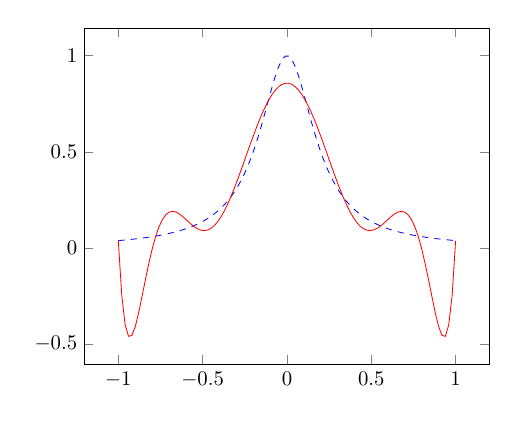
\begin{tikzpicture}[scale=0.75]
            \begin{axis}[xmin=-1,xmax=1,xmin=-1.2,xmax=1.2,samples=100]
                \addplot[domain=-1:1,blue,dashed]{1/(1+25*x*x)};
                \addplot[domain=-1:1,red,solid]{16.545674722429712 * x*x*x*x*x*x*x*x*x*x + 8.851286807773627e-13 * x*x*x*x*x*x*x*x*x + -12.079377458718012 * x*x*x*x*x*x*x*x + -1.6319051537287015e-12 * x*x*x*x*x*x*x + -22.778903788331114 * x*x*x*x*x*x + 8.747268893200492e-13 * x*x*x*x*x + 25.348331583973515 * x*x*x*x + -1.4087385060936399e-13 * x*x*x + -7.854564043148674 * x*x + 6.6005027351349585e-15 * x + 0.8573005222561162};
            \end{axis}
         \end{tikzpicture}
        \caption{پدیده‌ی رونگه}
        \label{fig:runge}
    \end{subfigure}
    \hfill
    \begin{subfigure}[b]{0.45\textwidth}
        \centering
        \begin{tikzpicture}[scale=0.75]
            \begin{axis}[xmin=-1,xmax=1,xmin=-1.2,xmax=1.2,samples=100]
                \addplot[mark=none,blue,dashed] table{\gibbsref};
                \addplot[mark=none,red,solid] table{\gibbs};
            \end{axis}
         \end{tikzpicture}
        \caption{پدیده‌ی گیبس}
        \label{fig:gibbs}
    \end{subfigure}
       \caption{دو پدیده‌ی رونگه و گیبس. در هر دو نمودار خم آبی تابع هدف و خم قرمز تقریب متناظر با آن تابع می‌باشد. (آ) تابع رونگه و تقریب آن توسط یک چندجمله‌ای درجه 10. (ب) تابع پله‌ای و تقریب آن با استفاده از 30 جمله‌ی اول سری فوریه‌ی متناظر آن.}
       \label{fig:runge_gibbs}
\end{figure}

همان گونه که در شکل نیز مشاهده می‌شود، پدیده‌ی رونگه تاثیر به مراتب مخرب‌تری از پدیده‌ی گیبس دارد. در واقع، می‌توان نشان داد که خطای درون‌یابی  در مثال بالا برابر با 
$O(2^n‌)$ 
است، در حالی که خطایی که پدیده‌ی گیبس در محاسبات وارد می‌کند 
$O(1)$ 
است. در پدیده‌ی رونگه، همان طور که قبلا نیز به آن اشاره شد، بیشترین میزان خظا در نزدیکی مرزهای دامنه‌ی ورودی تابع اتفاق می‌افتد. به عبارت دیگر، اگر دامنه‌ی ورودی بازه‌ی 
$[0,1]$ 
باشد، انتظار داریم ابعادی از ورودی که به مقادیر صفر یا یک نزدیک باشند بیشترین حساسیت را در خروجی تابع درون‌یاب به وجود بیاورند. در مقابل، در صورتی که با پدیده‌ی گیبس رو به رو باشیم، این حساسیت در قسمت‌هایی از سیگنال ورودی که ناپیوستگی وجود دارد به وجود می‌آید.

پدیده‌ی رونگه هنگام درون‌یابی با استفاده از چندجمله‌ای‌های درجه بالا بروز می‌کند. ولی اکثریت مدل‌های یادگیری ماشین، از جمله شبکه‌های عصبی، از پایه‌ی تک‌جمله‌ای درجه یک برای ورودی استفاده می‌کنند. با این وجود، این مدل‌ها به طرق مختلف برای یادگیری توابع غیرخطی تعمیم می‌یابند. در نتیجه، دور از ذهن نیست که پدیده‌ی رونگه، یا پدیده‌ی مشابهی، در این مدل‌ها وجود داشته باشد. برای محک زدن این ادعا، می‌توان آزمایش ساده‌ای طراحی کرد. در صورتی که با پدیده‌ی رونگه مواجه باشیم، تغییر تابع پایه‌ی تک‌جمله‌ای به پایه‌ی چبیشف، باید تاثیرات مشخصی در بهبود مقاومت شبکه در برابر حملات خصمانه و ماهیت این حملات داشته باشد. نتایج این آزمایش‌ها شواهد بسیار قویی در تایید ارتباط مثال‌های خصمانه و پدیده‌ی رونگه نشان می‌دهند. جزییات و نتایج این آزمایش‌ها را در بخشی جداگانه شرح و بسط می‌دهیم.

با توجه به اینکه بهبود مشاهده شده بدون تغییر در تابع هدف، روش آموزش یا تغییر فاکتور غیرخطی حاصل شده، دور از ذهن نیست که انتقال‌پذیری مثال‌های خصمانه حاصل از اصل داربو باشد. ابتدا اصل داربو را آن طور که در (کتاب) آمده بیان می‌کنیم.
\begin{theorem}[اصل داربو]
    در تمامی انواع بسط طیفی (از جمله سری‌های توانی عادی)، هم دامنه‌ی همگرایی در صفحه مختلط و هم نرخ همگرایی توسط مکان و قدرت بدترین تکینگی در صفحه‌ی مختلط تعیین می‌شود. در اینجا، منظور از تکینگی قطب‌ها، توان‌های کسری، لوگاریتم‌ها و دیگر نقاط شاخه و ناپیوستگی‌های تابع 
    $f(z)$ 
    یا هرکدام از مشتقات آن است.
\end{theorem}

از اصل داربو می‌توان قضیه‌ی فرعی زیر را مستقیما نتیجه گرفت.

\begin{corollary}
    اگر دو تابع 
    $f(z)$ 
    و 
    $g(z)$ 
    دارای تکینگی‌های یکسان محدود کننده‌ی همگرایی باشند، ضرایب مجانب بسط طیفی آن‌ها در حد
    $n \rightarrow \infty$ 
    برابر خواهد بود.
\end{corollary}

همان گونه که در (مقاله) ذکر شده است، مثال‌های خصمانه‌ی یک شبکه را می‌توان به شبکه‌ی دیگری که بر روی داده‌های آموزشی متفاوتی آموزش داده شده است منتقل کرد. با توجه به نتیجه‌ی مستقیم اصل داربو، انتقال‌پذیری مثال‌های خصمانه را می‌توان به وجود تکینگی‌ها در تابعی که قصد یادگیری آن را داریم نسبت داد. این موضوع توجیه قابل قبولی برای انتقال مثال‌های خصمانه بین شبکه‌های مختلف، که مستقل از داده‌های آموزشی استفاده شده است، ارائه می‌دهد. حال تعاریف لازم برای تشریح دلیل وجود مثال‌های خصمانه، چگونگی تاثیر آن‌ها بر خروجی شبکه و انتقال‌پذیری آن‌ها را داریم.

مثال‌های خصمانه نقاطی در همسایگی مثال‌های طبیعی در نزدیکی مرز دامنه‌ی ورودی شبکه هستند که خروجی شبکه در همسایگی این مثال‌ها نوسنات شدیدی ناشی از پدیده‌ی رونگه دارد. در نتیجه، با استفاده از اطلاعات گرادیان تابع در آن نقطه، می‌توان مثالی در همسایگی آن مثال طبیعی یافت که شبکه با اطمینان بالایی آن را اشتباه طبقه‌بندی می‌کند.

به عبارت دیگر، اکثر مثال‌های طبیعی در نزدیکی یا روی مرز دامنه‌ی ورودی هستند\footnote{به عنوان مثال، در 
\lr{MNIST} 
اکثر ابعاد ورودی مقدار ۰ یا ۱ را دارند که دقیقا بر روی مرز دامنه‌ی ورودی قرار گرفته است.}.
محدوده‌ی همگرایی بسط طیفی یادگیری شده در این نقاط بسیار کوچک است و با کمی جابه‌جایی می‌توان از این محدوده خارج شد. این مسئله، احتمالا در ابعاد بالا بسیار تشدید می‌شود، زیرا در ابعاد بالا اکثر جرم فضا در نوار نازکی اطراف مرز دامنه‌ی ورودی قرار گرفته است. با توجه به این موضوع، محتمل است که وجود اختلالات خصمانه‌ی جهانی، که در (مقاله) مطرح شده‌اند، ناشی از این توزیع شدن مثال‌های طبیعی در نزدیکی مرزها و وجود تقارن در پدیده‌ی رونگه باشد.

از آنجایی که تعداد پارامترهای شبکه‌های عصبی بسیار زیاد است، با استفاده از اصل داربو، می‌توان انتظار داشت که ضرایب مجانب بسط طیفی یادگیری شده برای این شبکه‌ها بسیار نزدیک یا برابر باشد. در نتیجه، تمامی این شبکه‌ها، بدون در نظر گرفتن معماری و مجموعه‌ی آموزشی استفاده شده، رفتار یکسانی در اطراف تکینگی‌ها نشان می‌دهند و به همین دلیل مثال‌های خصمانه‌ای که برای یکی از این شبکه‌ها ساخته می‌شود برای بقیه‌ی شبکه‌ها نیز خصمانه است.
\section{نتایج}
نتایج.

\end{document}